\documentclass[a4paper,12pt]{report}

\usepackage{alltt, fancyvrb, url}
\usepackage{graphicx}
\usepackage{geometry}
\usepackage[utf8]{inputenc}
\usepackage{float}
\usepackage{hyperref}



\usepackage[italian]{babel}

\usepackage[italian]{cleveref}

\title{\textbf{BREAKOUT}}
\author{Vincenzo Prisco\\
\texttt{vincenzo.prisco@studio.unibo.it}
\and Giacomo Ruscelli\\
\texttt{giacomo.ruscelli2@studio.unibo.it}
\and Sohail Mama\\
\texttt{sohail.mama@studio.unibo.it}
\and Yosberto Baro Carbonell\\
\texttt{yosberto.baro@studio.unibo.it}}
\date{\today}

\begin{document}

\maketitle
\newpage

\tableofcontents

\newpage

\chapter{Analisi}
Il software ha come obiettivo simulare il famosissimo gioco arcade prodotto da ATARI (nota casa produttrice di videogiochi statunitense), di nome Breakout che si basa sull’abilità del giocatore nel riuscire a rompere i mattoncini senza far cadere la palla al di sotto della barra.
\section{Requisiti}
\subsection{Requisiti funzionali}
\begin{itemize}
    \item L’utente aprendo il gioco dovrà muovere la barra a destra o a sinistra in base a dove l’utente prevede che la palla rimbalzerà, la palla rimbalzando sulla barra, tornerà in su seguendo una direzione dettata dal punto in cui rimbalza sulla barra e dovrà rompere più mattoncini possibili; il compito dell'utente è di mantenere almeno una palla in gioco per continuare a giocare.
\end{itemize}

\subsection{Requisiti non funzionali}
\begin{itemize}
    \item L'utente dovrà cercare di salvare più palle possibili cosi da avere più chance di distruggere tutti i mattoncini
\end{itemize}
\section{Analisi e modello del dominio}
L'utente dovrà essere in grado di capire la traiettoria della palla nel momento in cui colpendo i mattoncini scenderà, cosi facendo l'utente dovrà spostare la barra in modo che la palla non cada al di sotto della barra, nel caso in cui la palla rimbalza sulla barra, essa ritornerà in su verso i mattoncini, e così via fino alla distruzione di tutti i mattoncini.

\begin{figure}[htbp]
    \makebox[\textwidth][l]{%
        \hspace*{-1in} % Sposta l'immagine a sinistra
        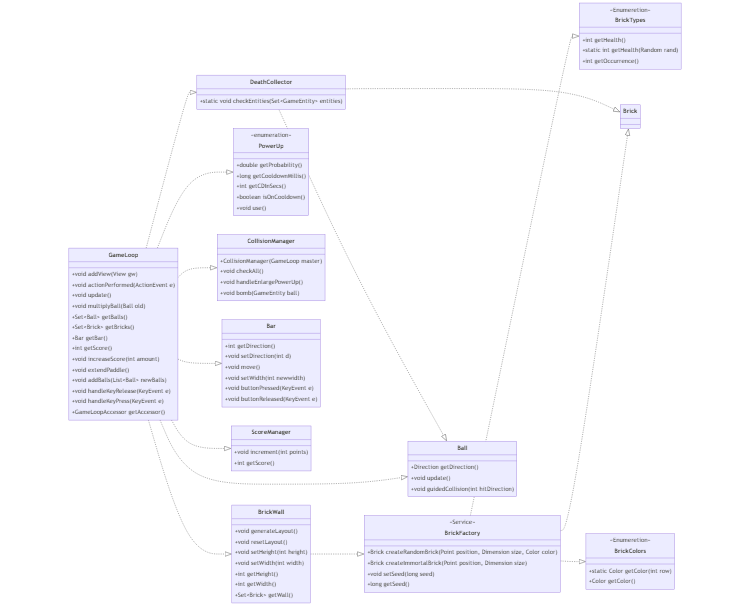
\includegraphics[width=1.5\textwidth]{total.png}}
    \caption{Modello del dominio}
    \label{fig:label}
\end{figure}


\chapter{Design}

\section{Architettura}
Per la realizzazione di "Breakout", è stato utilizzato il pattern architetturale MVC:
\begin{itemize}
    \item Model: si occupa di definire le varie entità del gioco, in particolare la palla (Ball), la barra (Bar), i mattoncini (con le classi Brick, BrickColors e BrickTypes), i bonus (BarExtender, Bomb) e la scoreboard.
    \item Controller: si occupa di definire il gameloop, creare i mattoncini attraverso la brickfactory, gestire il punteggio attraverso la classe ScoreManager, gestire i vari componenti che man mano "muoiono" attraverso la classe DeathCollector  e infine far partire il gioco attraverso la classe Match e Main.
    \item View: si occupa di tutto l'aspetto grafico, passando dal menu principale, alla view del gioco e della scoreboard.
\end{itemize}
In questo modo si ha una suddivisione delle classi in base alle funzionalità, ma allo stesso tempo si ha un aggiornamento delle entità utilizzate all'interno della view.

\section{Design Dettagliato}
\textbf{Sohail Mama}
\newline
\newline
\textit{Implementazione della musica di background e i suoni}
\newline
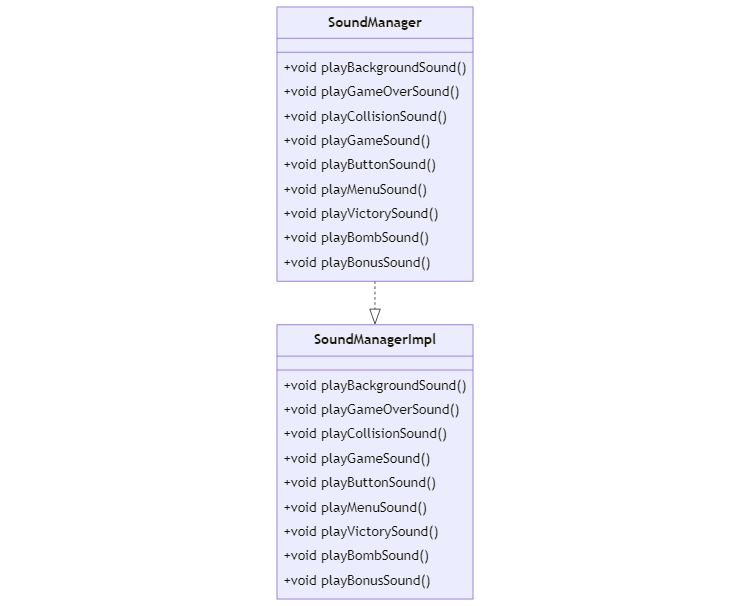
\includegraphics[width=\textwidth]{SoundManager.png}
\newline

\textbf{Problema:} implementare il suono all'interno del gioco, che sia per i bottoni, per il background o per le varie view
\newline
\newline
\textbf{Soluzione:} ho utilizzato il pattern facade all'interno del SoundManager, che semplicemente prende i vari file audio.wav, li passa ad un URL, cosicchè utilizzo l'URL passandolo all'AudioSystem creando così un'AudioClip, che verrà riprodotta ogni volta che il gameloop o le varie view richiameranno il metodo del SoundManager che contiene il suono desiderato.  
\newline
\newline
\textit{Implementazione della GameView}
\newline
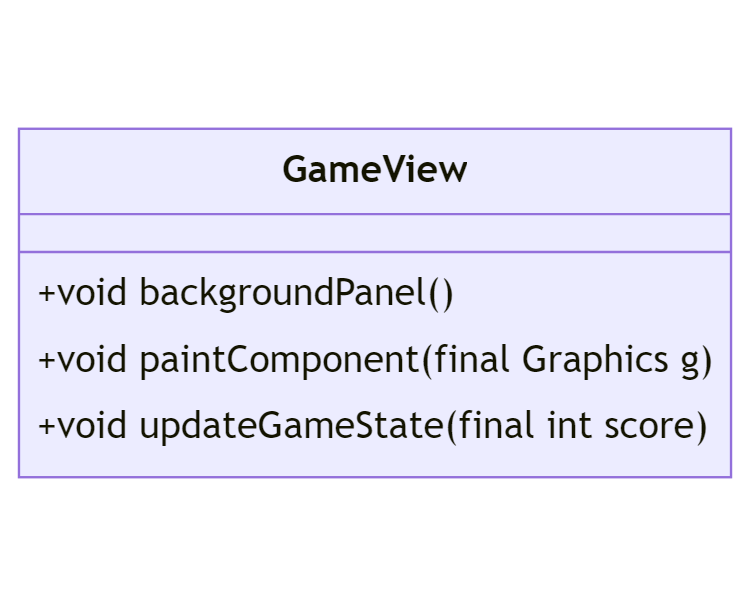
\includegraphics[width=\textwidth]{gameview.png}
\newline
\textbf{Problema:} disegnare i vari componenti del gioco su un background e farli aggiornare ogni Time Unit
\newline
\newline
\textbf{Soluzione:} ho utilizzato il pattern Observer all'interno della classe GameView, che disegna:
\begin{itemize}
    \item i brick passati tramite un for-each che itera sul brickWall, 
    \item la Bar
    \item la Ball
    \item il background che viene passato al metodo PaintComponent tramite il metodo backGroundPanel() che passa l'immagine ad un URL.
\end{itemize}
Invece per l'aggiornamento dello stato del gioco ho utilizzato updateGameState() che ridisegna tutti i componenti ogni time unit e in caso non ci siano più palline, crea un JContentPane che avvisa l'utente che ha perso, invece in caso non ci siano brick avvisa l'utente che ha vinto riproducendo rispettivamente il suono della sconfitta e quello della vittoria
\newline
\newline
\newline
\textbf{Vincenzo Prisco}
\newline
\newline
\textit{Implementazione del BrickWall}
\newline
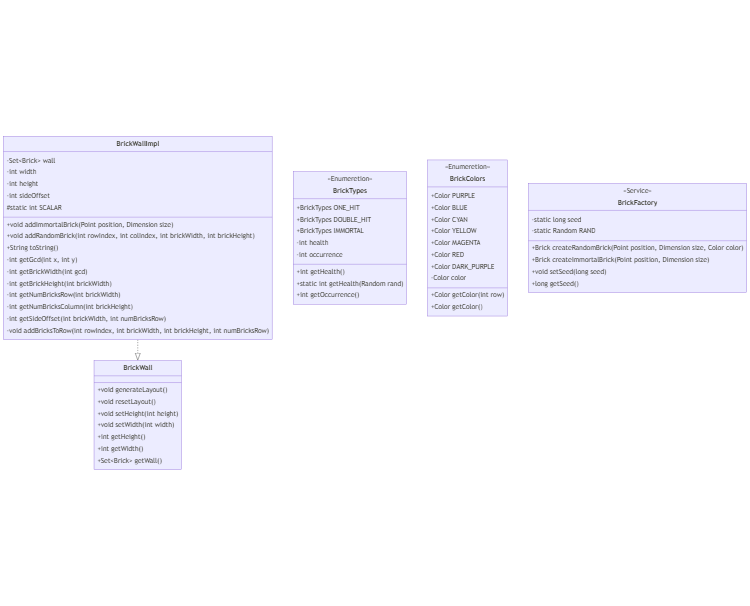
\includegraphics[width=\textwidth]{bricks.png}
\newline
\textbf{Problema:} Implementare un Muro di Mattoni generato randomicamente e proceduralmente
\newline

\newline
\textbf{Soluzione:} La classe BrickWallImpl viene inizializzata con le dimensioni dello spazio utile.\newline
Alla creazione del terreno di gioco, vengono presi i 2 valori di grandezza e utilizzati per ricavarne il GCD (Gratest Common Divisor). Con questo valore, utilizzato assieme all'Aspect Ratio definito all'interno della classe Brick, sara' facile ottenere l'altezza e la larghezza di ogni singolo mattone, mantenendo le proporzioni desiderate.
Per far si' che i valori ottenuti siano poi utilizzabili durante lo svolgimento (mattoni troppo piccoli o viceversa), il risultato viene moltiplicato per uno scalare.\newline
Successivamente all'aver ottenuto le dimensioni del mattone, si passa alla generazione del campo di gioco. Mattone per mattone viene chiamata la BrickFactory, che randomicamente fornira' il tipo di mattone da posizionare. Per questa scelta, si usufruisce dell'Enum BrickTypes, dove oltre a venir  definite le tipolige, viene anche registrata l'occorenza, dove i mattoni da 1 di vita avranno la priorita' su quelli immortali e con piu' vita. \newline
Tutti i Brick che avranno una vita maggiore di 0, avranno un colore proceduralmente scelto a seconda della loro posizione, noi abbiamo optato per un pattern ad onda, che si ripete per tutta l'altezza del muro. Tale comportamento e' gestito dall'Enum BrickColors.\newline
Nel caso ove, il GCD ottenuto, non sia in grado di riempire lo spazio per la sua larghezza, il campo in eccesso viene diviso per 2 e riempito con mattoni indistruttibili richiamando la BrickFactory.\newline
\newline
\textit{Gestione della morte delle palline e dei mattoni}
\newline
\newline
\textbf{Problema:} Come gestire la morte delle Palline e dei Mattoni
\newline
\newline
\textbf{Soluzione:} Dato che, entrambi i Model sono conservati in Set ed entrambi ereditano dalla classe astratta GameEntityImpl, e' stato semplicemente definita una classe chiamata DeathCollector, che si occupa di smaltire tutte le entita' presenti dentro un Set che hanno la loro vita uguale a 0 (non meno perche' -1 e' il valore usato per le entita' immortali)
\newline
\newline
\newline
\newline
\textbf{Yosberto Baro Carbonell}
\newline
\newline
\textit{Dare l’accesso ai vari GameEntity a molte classi in maniera safe}
\newline
\newline
\textbf{Problema:} Dare l’accesso ai vari GameEntity a molte classi in maniera safe.\newline
\textbf{Soluzione:} Implementazione del Pattern Facade e pattern \newline
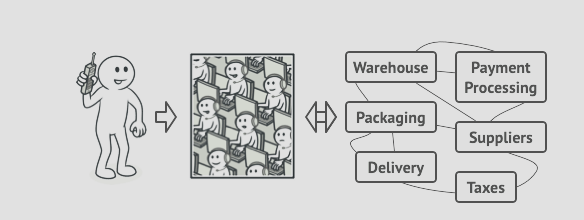
\includegraphics[width=\textwidth]{facadeExample.png}
``A facade is a class that provides a simple interface to a complex subsystem which contains lots of moving parts. A facade might provide limited functionality in comparison to working with the subsystem directly. However, it includes only those features that clients really care about."\newline
\footnote{\href{https://refactoring.guru/design-patterns/facade}{https://refactoring.guru/design-patterns/facade}}
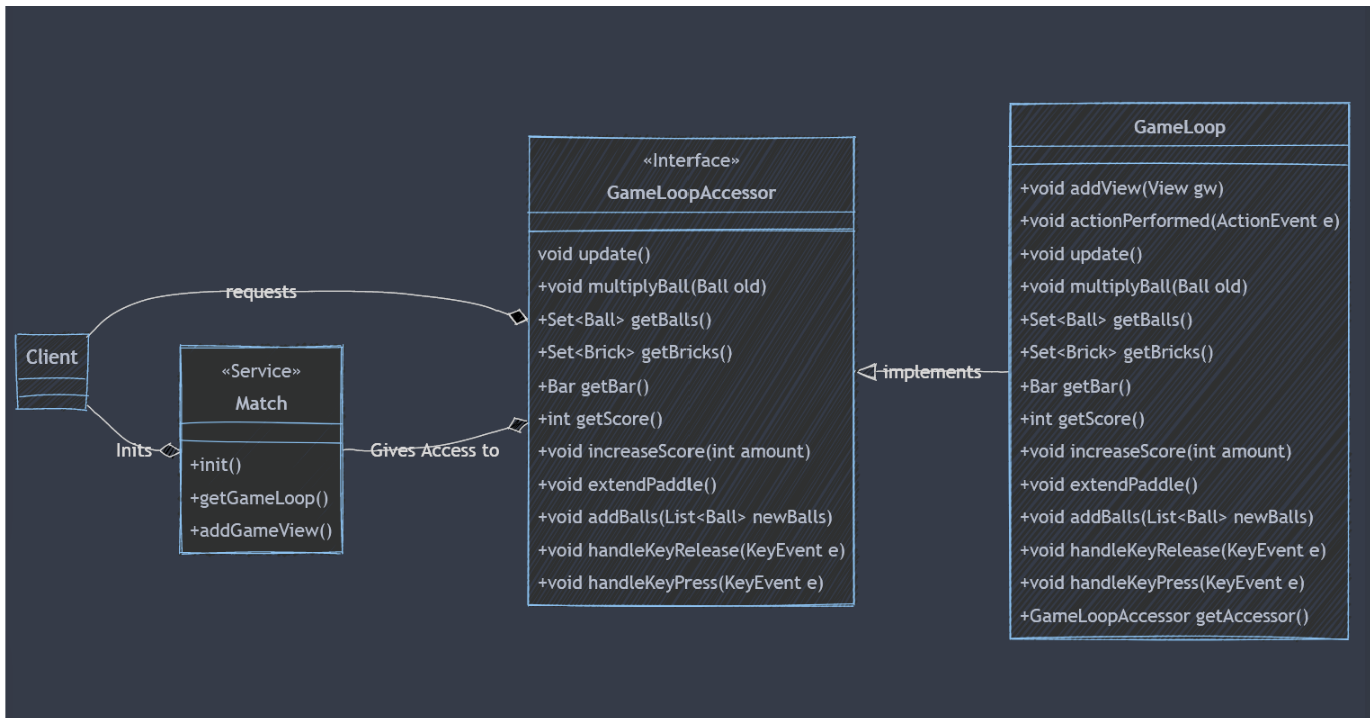
\includegraphics[width=\textwidth]{gameLoop.png}
Il GameLoop si occupa di tutta la business logic, provvedendo solo l’assolutamente necessario alle altri classi, e assicurandosi di dare dati non mutabili, il che permette a ogni classe di lavorarci senza preoccuparsi. Tuttavia questo non basta, vogliamo che ci sia solo un gameLoop, sempre, e vogliamo assicurarci che non possa essere usato male, per questo introduciamo GameLoopAccessor e l’utilizzo del pattern Singleton.
\newline
\newline
\textit{Garantire il controllo delle collisioni}\newline\newline
\textbf{Problema:} Garantire che il controllo delle collisioni tra gli oggetti del gioco sia gestito in maniera sicura ed efficiente.\newline
\textbf{Soluzione:} Implementazione di un sistema centralizzato di gestione delle collisioni \newline
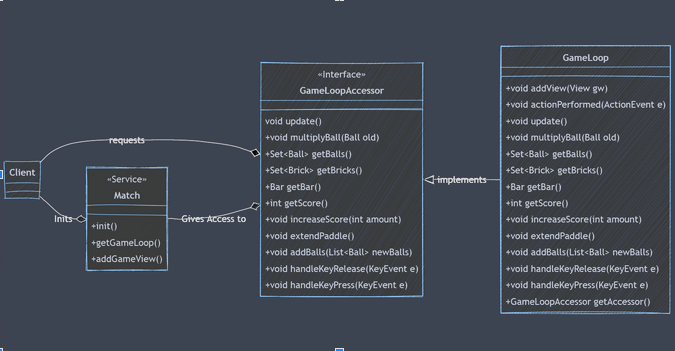
\includegraphics[width=\textwidth]{facadeSingleton.png}
La classe CollisionManager si occupa di tutta la logica relativa alle collisioni tra gli oggetti del gioco, come palline, mattoni e la barra. Essa verifica continuamente le collisioni e applica le conseguenze appropriate, come l'aggiornamento del punteggio o l'attivazione di potenziamenti. La classe CollisionManager utilizza un'istanza di GameLoopAccessor per accedere agli elementi del gioco in modo controllato, garantendo che i dati siano gestiti in modo sicuro e coerente.
Il CollisionManager utilizza tecniche di logging e misurazione del tempo per monitorare e ottimizzare le prestazioni delle verifiche di collisione, assicurandosi che il gioco rimanga fluido e reattivo, e permettendo un'identificazione veloce e reattiva in caso di problemi di performance.
\newline
\newline
\textit{Unire GameLoop e GameView in collaborazione con Sohail Mama}
\newline
\newline
\textbf{Problema: }Unire GameLoop e GameView \newline
\textbf{Soluzione:} Dato che utilizziamo già il modello MVC, ci siamo ispirati ai vecchi progetti in laboratorio che li dimostravano, e abbiamo creato un interfaccia View. Questo permette al GameLoop di semplicemente chiamare un metodo senza preoccuparsi di cosa fa nello spefico ogni View.
\newline
\newline
\newpage
\textbf{Giacomo Ruscelli}
\newline
\newline
All'interno del gruppo di lavoro il mio compito era quello di gestire la "barra" comandata dall'utente prendendo in input i comandi dell'utente; mi sono anche occupato della gestione della classifica tramite l'interazione con un file locale in formato Json usato come database, infine ho gestito l'implementazione del power up bomba


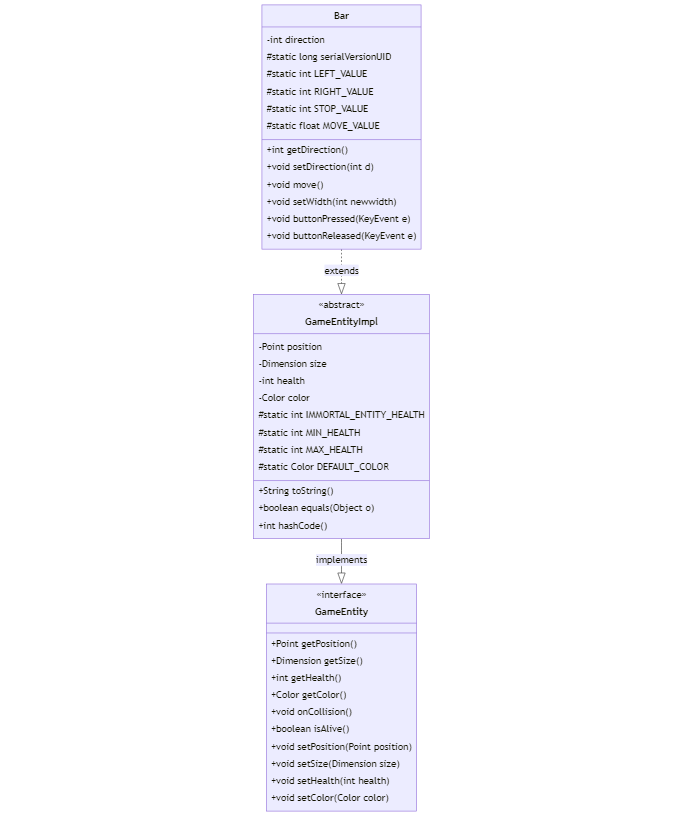
\includegraphics[width=\textwidth]{Bar.png}\newline

{\textbf{Problema:}} La classe Bar rappresenta una barra mobile all'interno di un gioco. Questa barra può muoversi a sinistra e a destra in risposta agli input dell'utente tramite la tastiera. Il problema affrontato da questa classe include: Movimento della barra, Gestione degli input della tastiera e Modifica della dimensione della barra.
\newline
\begin{enumerate}
\item \textbf{Movimento della barra}: Aggiornare la posizione della barra in base alla direzione determinata dagli input dell'utente
\item \textbf{Gestione degli input della tastiera}: Rilevare quando l'utente preme o rilascia i tasti freccia sinistra e destra per determinare la direzione del movimento della barra.
\item \textbf{Modifica della dimensione della barra}: Consentire la modifica della larghezza della barra durante il gioco, ad esempio per effetto di power-up. 
\end{enumerate}
{\textbf{Soluzione:}}
\begin{enumerate}
\item \textbf{Movimento della barra}: La direzione della barra viene memorizzata nella variabile "direction" (destra o sinistra). Il metodo move aggiorna la posizione della barra ad ogni ciclo di gioco in base al valore della direzione. Se la direzione è sinistra, la barra si sposta verso sinistra; se la direzione è destra, la barra si sposta verso destra; se la direzione è zero, la barra rimane ferma. Il movimento viene limitato all'interno dei limiti di gioco. \newline
\item \textbf{Gestione degli input della tastiera}: La classe utilizza due mappe (KEY\_PRESSED\_ACTIONS e KEY\_RELEASED\_ACTIONS) per associare i codici dei tasti delle frecce sinistra e destra a delle funzioni lambda che aggiornano la direzione della barra. Ad ogni rilascio e pressione di un tasto della tastiera si controlla se corrisponde a quelli mappati e si esegue il comando corrispondente.
\item \textbf{Modifica della dimensione della barra}: Per consentire la modifica della dimensione ho inserito nella classe Bar un metodo utile a settare la dimensione.\newline \newline
\end{enumerate}
\textbf{Scoreboard}\newline \newline
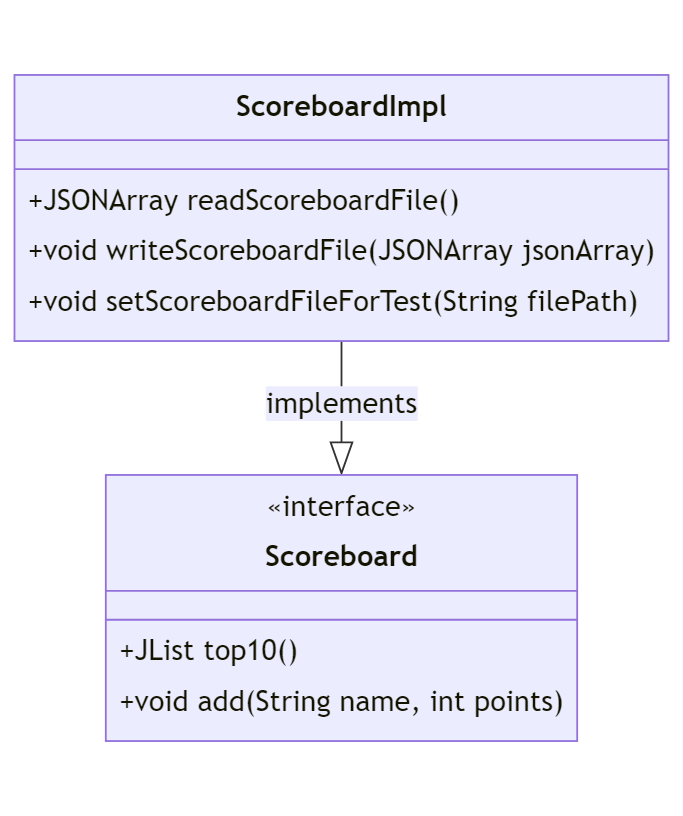
\includegraphics[width=\textwidth]{Scoreboard.png}
\textbf{Descrizione del Problema:} La classe Scoreboard gestisce la classifica dei punteggi realizzati dagli utenti memorizzandolo in un file JSON. Di seguito è riportata un'analisi dei problemi specifici affrontati e delle soluzioni implementate: \newline
\begin{enumerate}


\item \textbf{Lettura e Scrittura dei Dati JSON:} Leggere e scrivere dati da/in un file JSON all'interno di un archivio JAR.
\item \newline \textbf{Creazione della Lista dei Migliori 10 Giocatori:} Estrarre e formattare correttamente i primi 10 giocatori in base al punteggio da un JSONArray.
\item \newline \textbf{Aggiunta di nuove voci alla classifica:} Gestire l'aggiunta di nuove voci alla classifica esistente, garantendo che siano correttamente ordinate.\newline \newline
\end{enumerate}
\textbf{Soluzione adottata:} \newline

\begin{enumerate}

\item \textbf{Lettura e Scrittura dei Dati JSON:} La classe gestisce la lettura da un file JAR usando un sistema di file dinamico se necessario, assicurando che i dati siano accessibili e modificabili.

\item \textbf{Creazione della Lista dei Migliori 10 Giocatori:} Utilizza Java streams per ordinare e formattare i dati in una lista di stringhe (\texttt{JList<String>}), garantendo una visualizzazione chiara e ordinata dei risultati.

\item \textbf{Aggiunta di nuove voci alla classifica:} Legge il punteggio corrente, aggiunge la nuova voce, ordina il punteggio in base ai punti e sovrascrive il file JSON con i dati aggiornati.

\end{enumerate}
\textbf{Power up bomba}\newline
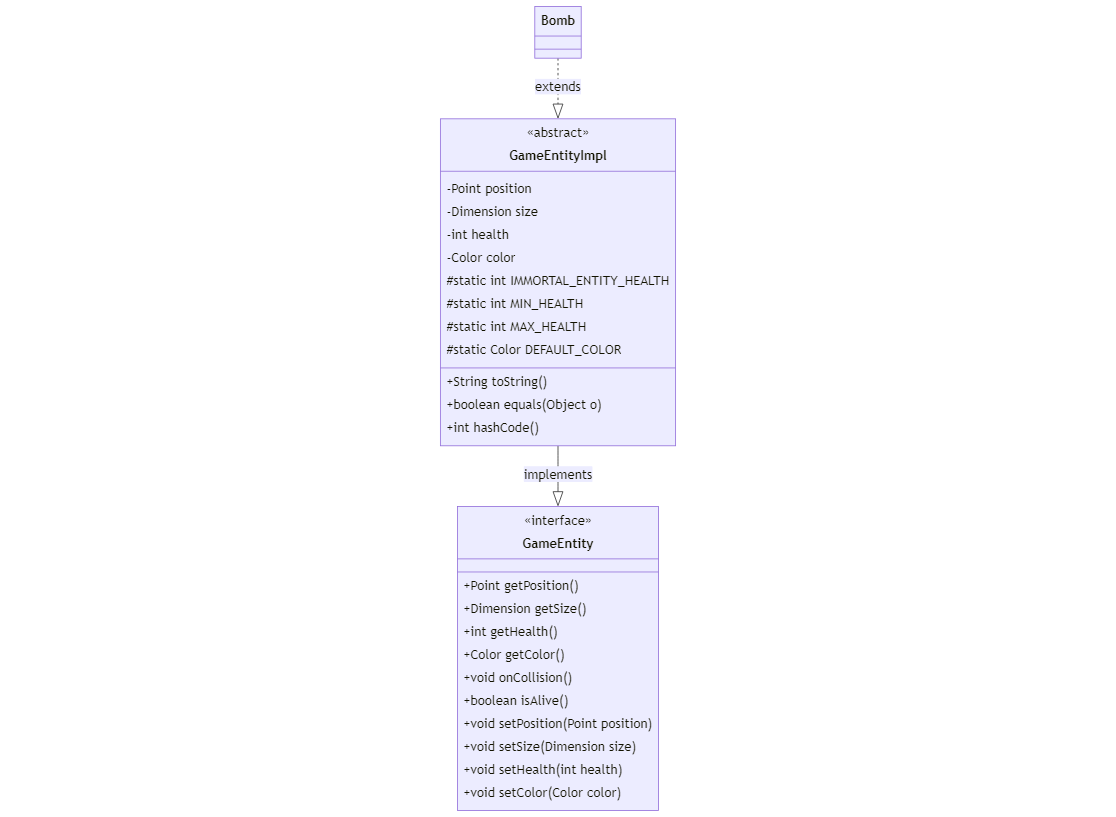
\includegraphics[width=\textwidth]{bomb.png}\newline
\textbf{Descrizione del Problema.} La classe deve implementare il power up bomba, garantendone la corretta funzionalità senza appesantire e rallentare il programma.\newline
\begin{enumerate}
\item \textbf{Ottimizzazione:} bisogna garantire fluidità nel codice e di conseguenza è necessario garantire l'ottimizzazione massima
\item \textbf{Scelta della dimensione:} la dimensione della bomba non potrà risultare arbitraria, bisogna valutare la dimensione a seconda dell'area di gioco
\item \textbf{Logica:} come gestire il codice dietro l'esecuzione del power up
\end{enumerate}
\textbf{Soluzioni adottate.} \newline

\begin{enumerate}
\item \textbf{Ottimizzazione:} per otimizzare il codice ho deciso di creare un quadrato e di controllare l'intersezione di ogni mattone con esso, se si intersecano allora il cubetto viene colpito dall'esplosione e danneggiato/distrutto, il codice è integrato nel collision manager
\newline
\item \textbf{Scelta della dimensione:} la dimensione è decisa a seconda della dimensione della schermata di gioco, si è scelto che la dimensione dei lati sarà di 1/5 l'area di gioco
\item \textbf{Logica:} all'interno del collision manager è stato inserito un pezzo di codice che gestisce l'avvenimento del power up bomba, viene gestito come se ci fosse una grande palla fissa all'interno del gioco a cui vengono controllate le collisioni e applicate gli effetti delle collisioni ai brick interessati.
\end{enumerate}
\chapter{Sviluppo}
\section{Testing automatizzato}
Per il testing automatizzato abbiamo utilizzato JUnit nella versione 5.10.1.\newline
Ogni interfaccia implementata possiede il suo corrispettivo test,
\section{Note di sviluppo}
\textbf{Yosberto Baro Carbonell}\newline
\href{https://github.com/Carbocode/OOP23-Breakout/blob/5098fbc11d7a6030a018341082738afb8926974c/src/main/java/it/unibo/controller/GameLoop.java\#L148}{Utilizzo di thread e timer per GameLoop}\newline
\href{https://github.com/Carbocode/OOP23-Breakout/blob/5098fbc11d7a6030a018341082738afb8926974c/src/test/java/it/unibo/api/CollisionManagerTest.java\#L89}{Utilizzo di Stream per selezionare oggetto random da un Set}\newline
\newline
\textbf{Giacomo Ruscelli}\newline
\href{https://github.com/Carbocode/OOP23-Breakout/blob/69327514cd4e3f224d6867c94b9345083c8b08f5/src/main/java/it/unibo/model/Bar.java\#L130}{Utilizzo di Lambda expression}\newline
\href{https://github.com/Carbocode/OOP23-Breakout/blob/69327514cd4e3f224d6867c94b9345083c8b08f5/src/main/java/it/unibo/model/ScoreboardImpl.java\#L98}{Utilizzo di Stream}\newline
\href{https://github.com/Carbocode/OOP23-Breakout/blob/69327514cd4e3f224d6867c94b9345083c8b08f5/src/main/java/it/unibo/model/Bar.java\#L36}{Utilizzo mappa per associare tasti con lambda expression}
\newline
\newline
\textbf{Sohail Mama}\newline
\href{https://github.com/Carbocode/OOP23-Breakout/blob/4f84e369afabdf19194b28f7ea207b114760d0c7/src/main/java/it/unibo/view/GameView.java#L153}{Utilizzo lambda e stream}

\chapter{Considerazione finali}
\textbf{Sohail Mama}\newline
Mi ritengo soddisfatto del lavoro che è stato fatto, ho imparato moltissime cose nuove, ma soprattutto ho imparato a lavorare di squadra, cosa che non avevo ancora fatto, poichè mi son approcciato a questo mondo da soli due anni.\newline
Il progetto a mio avviso è stato ben strutturato e molto interessante.\newline\newline
\textbf{Vincenzo Prisco}\newline
Lavorare con il pattern MVC in Java è stato davvero interessante. La suddivisione chiara delle responsabilità tra Modello, Vista e Controller ha reso il codice più ordinato e comprensibile. Questo approccio ha reso più semplice gestire le diverse parti dell'applicazione e ha favorito una migliore organizzazione del lavoro.\newline

Durante lo sviluppo del progetto, ho avuto l'opportunità di simulare dinamiche aziendali, coordinando le attività tra i vari moduli come farebbe un team di sviluppo in un contesto lavorativo. Questa esperienza mi ha fatto capire quanto sia importante la collaborazione e la comunicazione all'interno di un gruppo di lavoro, sottolineando l'importanza di una pianificazione accurata e di una comunicazione efficace per il successo del progetto.\newline

Per quanto Java sia stato un linguaggio affidabile per il progetto, rispetto a linguaggi come C\#, potrebbe mancare di alcune semplificazioni che potrebbero rendere il codice più leggibile e conciso.\newline

In conclusione, lavorare su questo progetto mi ha arricchito professionalmente, migliorando le mie competenze nello sviluppo software e preparandomi per affrontare sfide più complesse in futuro. La combinazione di apprendimento pratico e simulazione delle dinamiche aziendali è stata un'esperienza formativa che mi ha permesso di crescere come sviluppatore e di apprezzare l'importanza della progettazione e della collaborazione nel mondo del software.\newline\newline
\textbf{Yosberto Baro Carbonell}\newline
Nel complesso, ritengo che il nostro gruppo abbia lavorato in modo efficace e rapido durante le sessioni in presenza, specialmente quando il progetto ha iniziato a prendere slancio. Tuttavia, il lavoro online si è rivelato più difficile, poiché non era possibile fornirci supporto e consigli con la stessa efficacia. 
Personalmente, ho trovato il progetto molto interessante, poiché mi ha permesso di utilizzare framework e tecnologie di cui non ero a conoscenza. Anche se non tutte quelle esplorate sono state incluse nel progetto finale. SpotBugs, in particolare, mi ha aiutato a individuare errori di cui non ero consapevole e, nel risolverli, ho acquisito una comprensione più profonda di concetti importanti della programmazione a oggetti, che in precedenza consideravo semplici formalità. Nonostante inizialmente fossi scettico e pensavo fosse troppo severo, ora riconosco l'importanza di scrivere codice pulito, corretto e sicuro, e ritengo che questa esperienza mi abbia reso un programmatore migliore, non solo in Java, ma in generale, poiché applicherò queste lezioni anche in futuro.
L'uso di Git è stato inizialmente complesso, ma dopo una o due settimane è diventato quasi una seconda natura. La creazione delle interfacce e la progettazione delle loro interazioni sono state le parti più coinvolgenti per me, insieme alla realizzazione del GameLoop. Lavorare sul GameLoop e sul CollisionManager mi ha permesso di contribuire a una parte fondamentale del gioco, coinvolgendomi in quasi tutte le fasi del progetto, sia per coordinare sia per offrire supporto. Questa esperienza mi ha fatto apprezzare molto il lavoro di gruppo e le sue sfide.
Venendo dal C\#, spesso ho sentito la mancanza delle sue funzionalità convenienti e della sua semplicità. Tuttavia, lavorare senza di esse si è rivelato benefico per il mio sviluppo come programmatore, poiché mi ha fatto capire quanto dipendessi da queste caratteristiche.
La parte più interessante del progetto è stata sicuramente lo studio dei design pattern. Questa esperienza complessiva non solo ha migliorato le mie competenze tecniche, ma mi ha anche insegnato l'importanza della collaborazione e dell'adattabilità nel lavoro di gruppo.\newline\newline
\textbf{Giacomo Ruscelli}\newline
In conclusione partecipare allo sviluppo di questo progetto ha significativamente potenziato le mie competenze tecniche e la mia capacità di lavorare efficacemente in ambiente Git, con non poche complicazioni dato che era la prima volta in cui utilizzavo così intensamente Git. Inoltre applicare le conoscenze teoriche acquisite durante il corso direttamente nella pratica su un progetto concreto ha consolidato il mio apprendimento, migliorando la mia capacità di progettare soluzioni software robuste e di collaborare in modo efficiente con altri sviluppatori.
\chapter{Guida Utente}
All'avvio dell'applicazione si ha un interfaccia Menu, per giocare bisogna premere con il mouse il bottone PLAY, per iniziare il gioco oppure SCOREBOARD per vedere la scoreboard
\newline
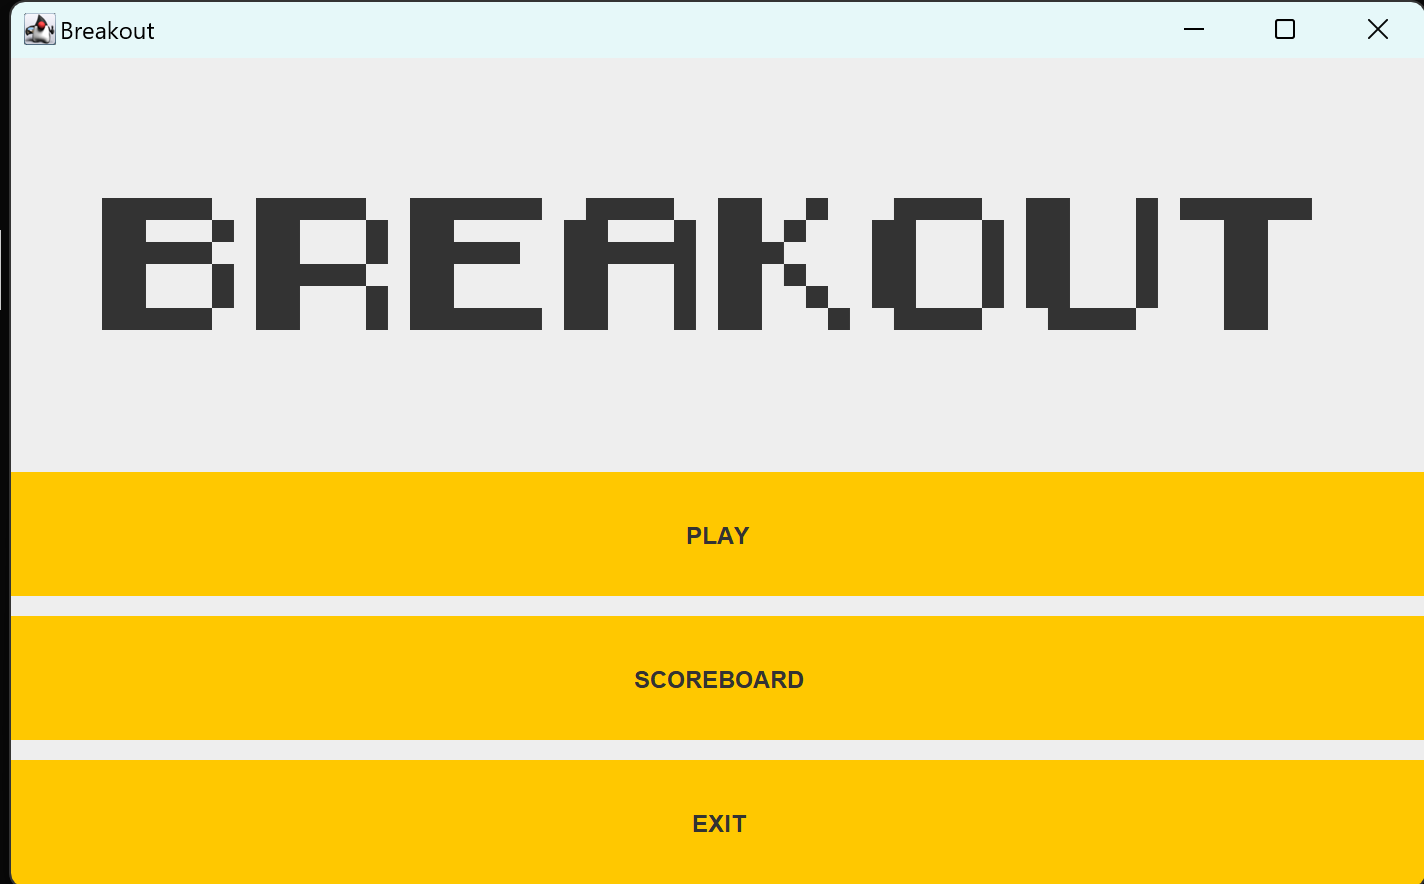
\includegraphics[width=\textwidth]{Menu.png}
\newline
Per giocare bisogna cliccare la freccetta destra o sinistra per muovere la barra che dovrà impedire alla palla di cadere
\newline
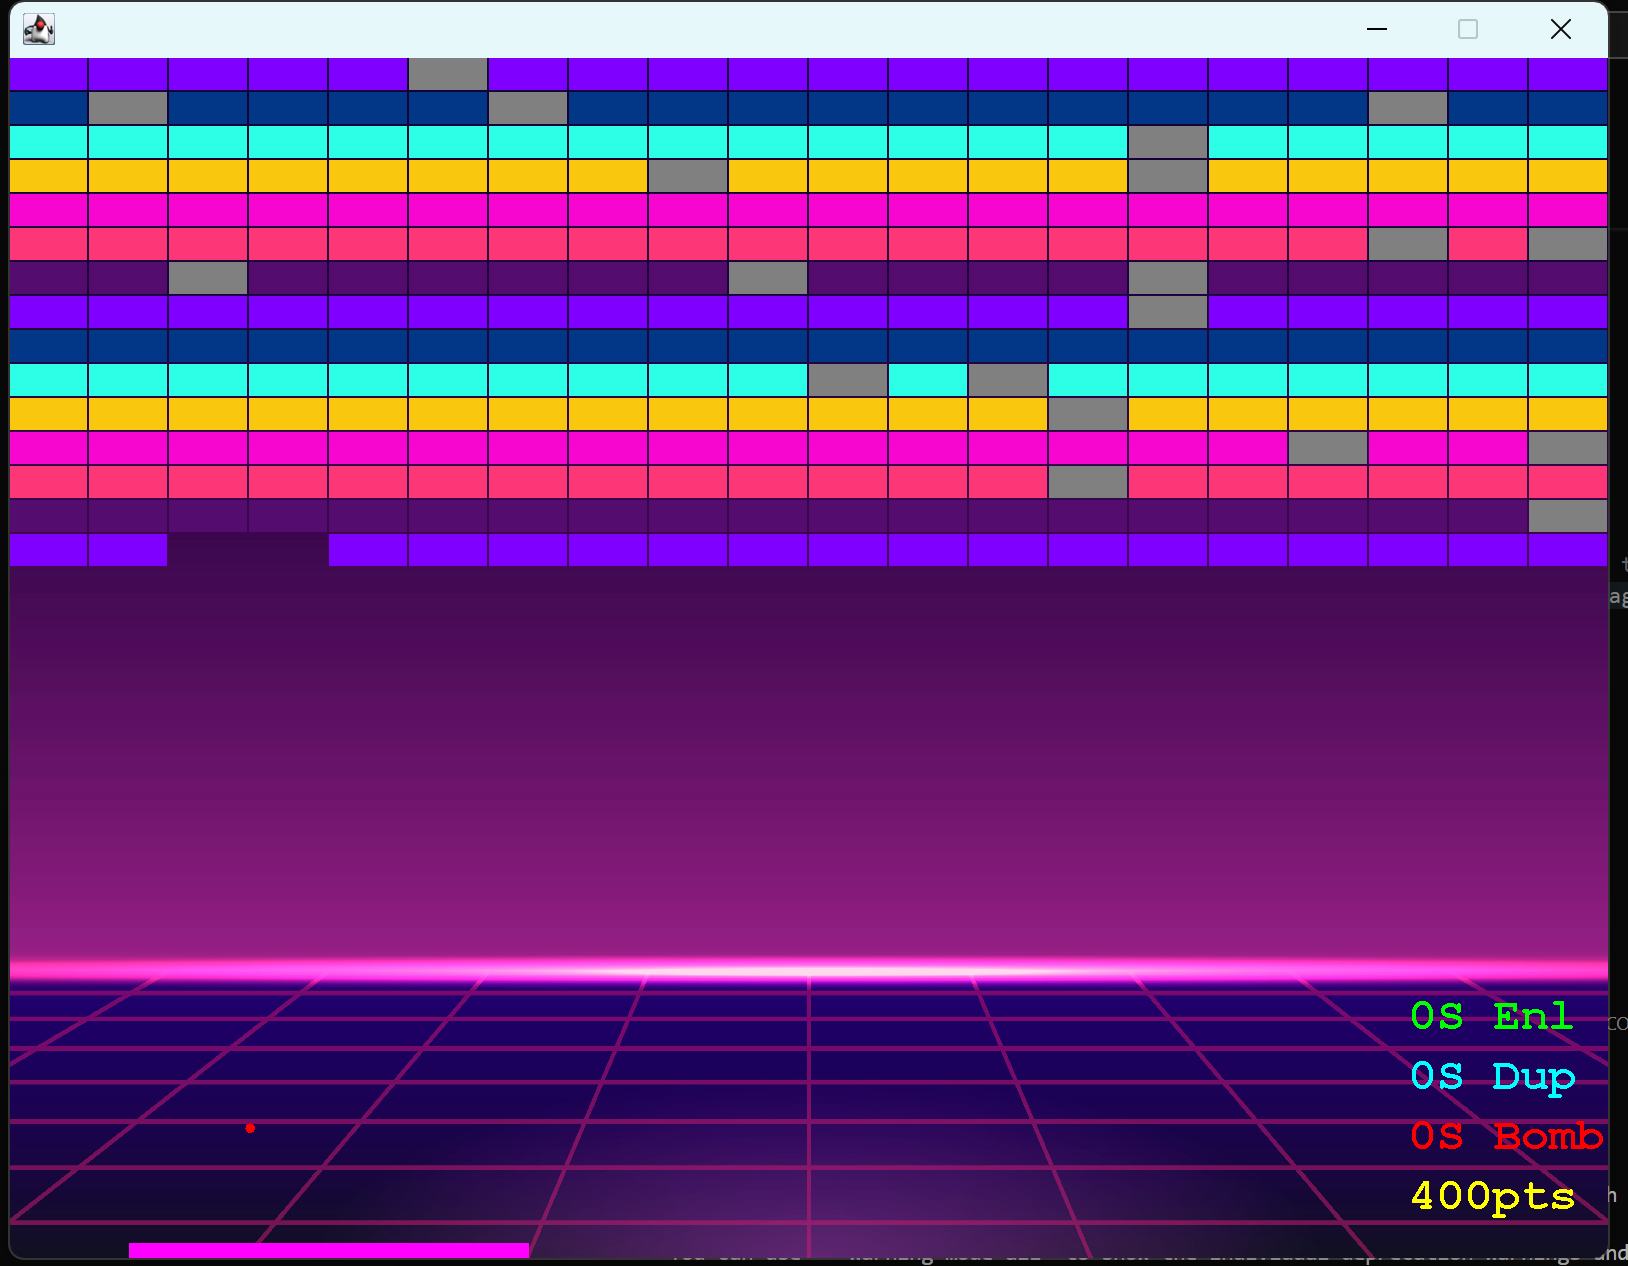
\includegraphics[width=\textwidth]{Game.png}
\newline
Il tuo obiettivo è distruggere più mattoni possibili
\newline
\newline
BUONA FORTUNA CAMPIONE!!!!
\end{document}